
\documentclass[11pt,a4paper]{article}

\usepackage[T1]{fontenc}
\usepackage[utf8]{inputenc}
\usepackage{lmodern}
\usepackage[a4paper,margin=2.4cm,top=2.3cm,bottom=2.3cm]{geometry}
\usepackage{graphicx}
\usepackage{booktabs}
\usepackage{caption}
\usepackage{float}
\usepackage{enumitem}
\usepackage{microtype}
\usepackage{xcolor}
\usepackage{fancyhdr}
\usepackage{titlesec}
\usepackage[hidelinks]{hyperref}

\definecolor{ink}{HTML}{14171A}
\definecolor{muted}{HTML}{6B6F6A}
\definecolor{rule}{HTML}{DCDDD7}

\captionsetup{font=small,labelfont=bf,textfont=small,skip=5pt}
\captionsetup[table]{position=top}
\setlength{\parindent}{0pt}
\setlength{\parskip}{5pt}
\setlength{\emergencystretch}{2.5em}
\renewcommand{\arraystretch}{1.12}

\titleformat{\section}{\Large\bfseries}{\thesection}{0.6em}{}
\titleformat{\subsection}{\large\bfseries}{\thesubsection}{0.5em}{}
\titleformat{\subsubsection}{\normalsize\bfseries}{\thesubsubsection}{0.5em}{}
\titlespacing*{\section}{0pt}{16pt}{5pt}
\titlespacing*{\subsection}{0pt}{11pt}{3pt}

\pagestyle{fancy}
\fancyhf{}
\renewcommand{\headrulewidth}{0.3pt}
\fancyhead[L]{\footnotesize\color{muted}PathSnap: Distributed Map-Matching and Route Reconstruction}
\fancyhead[R]{\footnotesize\color{muted}\thepage}
\begin{document}\thispagestyle{empty}
\begin{center}
\vspace*{2.4cm}
{\footnotesize\scshape PES University \quad Department of Computer Science and Engineering \quad RR Campus}

\vspace{1.8cm}
{\Huge\bfseries PathSnap}\\[8pt]
{\LARGE\bfseries Distributed Map-Matching and Route Reconstruction}

\vspace{0.7cm}
{\color{rule}\rule{0.45\textwidth}{0.4pt}}
\vspace{0.7cm}

{\large Reconstructing the road a vehicle actually drove from noisy GPS observations, using a
candidate classifier and a Viterbi decoder over the road network.}

\vspace{2.0cm}
\begin{tabular}{@{}ll@{}}
\textbf{Course} & UE24CS352A Machine Learning \\
\textbf{Team} & 174 \\
\textbf{Repository} & \url{https://github.com/shakthi-raja/pathsnap} \\
\textbf{Partitions} & 80 training, 10 student-testing, 10 reserved evaluator trips \\
\end{tabular}

\vspace{1.1cm}
{\small
\begin{tabular}{@{}p{0.12\textwidth}p{0.24\textwidth}p{0.26\textwidth}p{0.30\textwidth}@{}}
\textbf{Person} & \textbf{USN} & \textbf{Name} & \textbf{Contribution} \\
\midrule
1 & PES1UG24CS669 & KAVANA P G & Data reading, road network, candidates, features, alignment \\
2 & PES1UG25CS804 & ANUVIDYA R & Model training, comparison and Bayesian optimisation \\
3 & PES1UG24CS670 & KRUTHIKA C B & HMM and Viterbi decoding, FastAPI backend \\
4 & PES1UG25CS843 & SHAKTHI RAJA G P & Evaluator interface, Folium maps, integration, report \\
\end{tabular}
}

\vfill
{\footnotesize\color{muted}\today}
\end{center}
\clearpage
\section*{Abstract}
PathSnap matches noisy GPS observations to a road network and rebuilds the route a vehicle took. The dataset holds 90 trips from 77 locations on six continents, which rules out any global coordinate frame and any feature tied to one city. We score candidate road segments with a binary classifier over scale-free geometric features, then decode a connected path with Viterbi over the road graph. Five model families were compared under grouped cross-validation. The shipped model is HistGradientBoosting, with a student-test Top-1 accuracy of 81.6\% and log loss 0.168. On the ten reserved evaluator trips the decoder averaged 89.9\% pointwise accuracy, improving on the classifier alone on every trip.

\clearpage
\tableofcontents
\clearpage

\section{Introduction}

A GPS receiver in a city reports positions that wobble around the true path. Buildings reflect
signals, tunnels and underpasses break reception, and a 1\,Hz receiver can place a moving car on a
parallel street. Map matching is the task of recovering the road a vehicle actually used from that
noisy record.

The dataset supplies, for each trip, a GPS trace, a local road network given as nodes and directed
arcs, and a reference route expressed as an ordered list of arc identifiers. The reference route is
a sequence, not a label per observation, and that shapes the whole approach. The supervised target
has to be constructed, and it has to be constructed carefully enough that a wrong target is never
produced.

This report covers the data audit, the modelling decisions and the evidence behind them, the
sequential decoder, and the deployed two-laptop system. Every number in it comes from a file in the
repository, produced by the commands listed in Section~\ref{sec:reproduce}.

\section{Dataset understanding and exploratory data analysis}

The material was treated as a hypothesis rather than as fact. All 90 trips were audited before any
pipeline code was written, because a mistaken assumption there propagates into every result that
follows.

\subsection{Structure and partitions}

Each trip folder holds four tab separated files without headers: \texttt{.track} with longitude,
latitude and a timestamp in seconds; \texttt{.nodes} with node coordinates, where the row index is
the node identifier; \texttt{.arcs} with directed from and to node identifiers, where the row index
is the arc identifier; and \texttt{.route} with the reference sequence of arc identifiers. The 80
training trips are used for fitting and cross-validation, the 10 student-testing trips for
development comparison, and a further 10 reserved trips for final evaluation only.

\subsection{Audit findings}

Four findings changed the design.

The trips are not confined to one city. They span 77 distinct locations on six continents, from
$34^{\circ}$ south to $61^{\circ}$ north. A feature built on absolute coordinates would memorise a
city and fail everywhere else, and no single projected coordinate system is correct across the set,
so each trip is projected into its own local metric frame.

The median distance from an observation to the nearest road is 4.2 metres, with a 90th percentile of
6.0 metres. That justifies a 50 metre candidate radius with evidence rather than assumption.

Networks are large. The median trip carries 18,762 arcs and the largest carries 307,392, so
candidate search needs a spatial index.

The reference route does not always describe the whole drive. In 23 trips it covers less than 70
percent of the track length, and three trips are badly broken, with usable coverage of 14, 29 and 86
percent.

\begin{figure}[H]
\centering
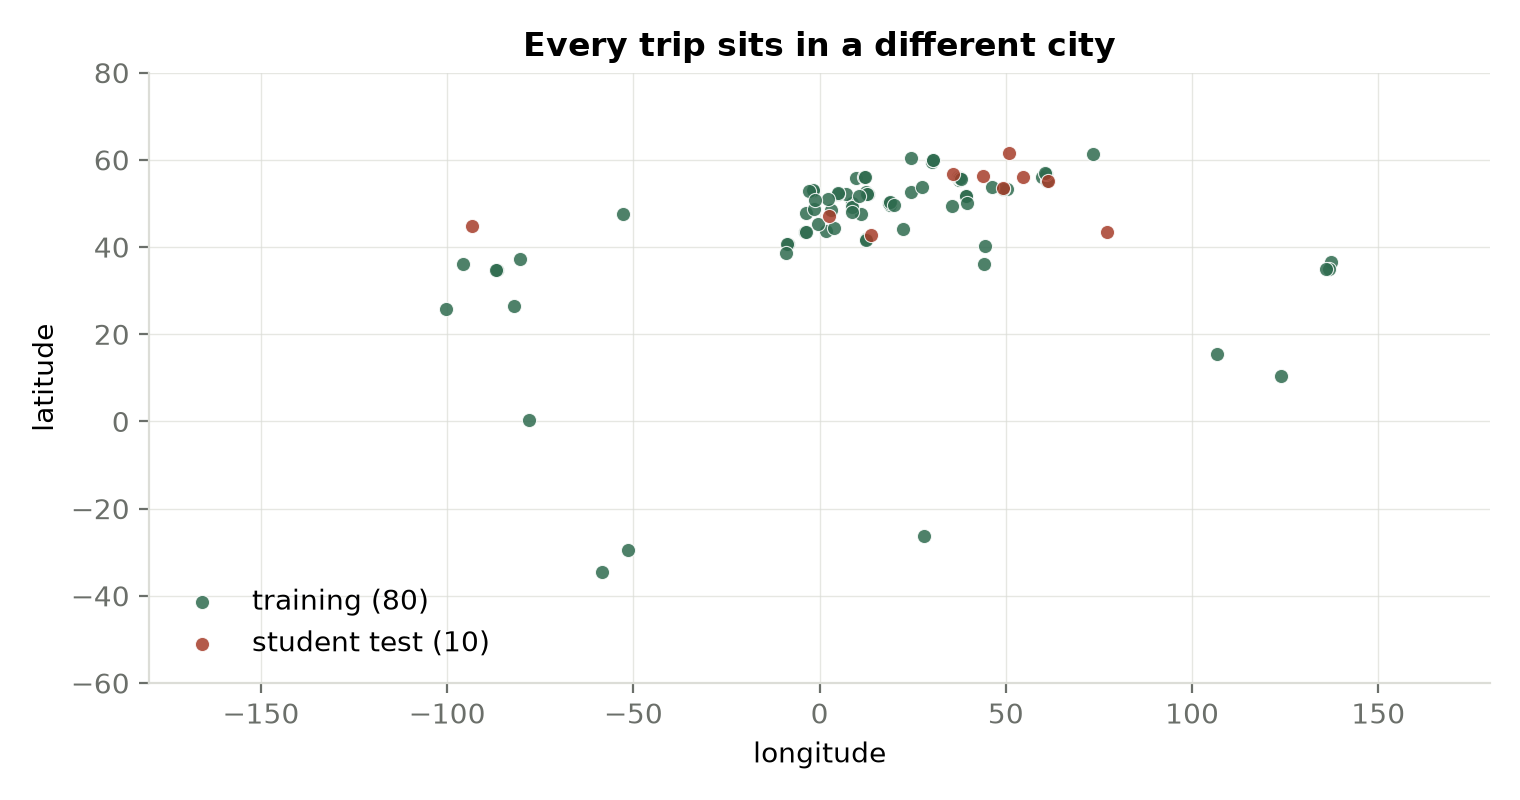
\includegraphics[width=0.9\textwidth]{figures/fig_trip_locations.png}
\caption{Location of every trip in the dataset. Latitude spans 35 degrees south to 62 north, so
grouped cross-validation over trips is cross-city validation rather than a random split.}
\label{fig:locations}
\end{figure}

That last finding matters more than it looks. A reference route covering only part of a drive cannot
supply a label for observations outside it, and forcing one would teach the model to be wrong with
confidence. The alignment stage therefore marks each observation as confident or unlabelled, and only
confident observations are used for supervision.

\subsection{Sampling intervals and missing values}

Two checks belong to the same audit. The first is how often the receiver reports. Across the 80
training tracks there are 208,417 observations and 201,051 consecutive gaps, of which 96.50\% are one second, 2.91\% span two to five seconds, 0.55\% span six to sixty seconds and 0.03\% exceed a minute. A trace that is mostly 1\,Hz with a thin tail of dropouts is where
simple interpolation breaks down and a decoder that scores transitions between observations helps. The same audit found no
non-finite longitude, latitude or timestamp in the raw tracks.

The second is how much of that signal can be supervised. Of the 208,417 observations, 90,043 (43.2\%) received a confident label from the alignment and 118,374 were withheld. That is a large fraction to leave unlabelled. The decision is deliberate. The
withheld observations fall where the reference route covers only part of the drive or where two arcs
are equally plausible, so labelling them would inject noise rather than signal.

Table~\ref{tab:missing} accounts for missing values. Both labelled partitions are covered, and every
candidate row in them is counted, including rows the model never sees. Every feature is complete
except for the first fix of a trip and for fixes that did not move. Nothing is imputed by hand. Each
pipeline carries a median imputer fitted inside its training fold.

\begin{table}[H]
\centering
\caption{Missing values per feature, as a share of all candidate rows in each partition. The remaining
eleven features are complete in both partitions.}
\label{tab:missing}
\small
\begin{tabular}{@{}lllp{0.44\textwidth}@{}}
\toprule
\textbf{Feature} & \textbf{Train} & \textbf{Student test} & \textbf{Cause} \\
\midrule
\texttt{movement\_m} & 0.05\% & 0.05\% & First observation of each trip has no predecessor. \\
\texttt{dt\_s} & 0.05\% & 0.05\% & Same rows: elapsed time is undefined without a previous fix. \\
\texttt{speed\_mps} & 0.05\% & 0.05\% & Same rows as the elapsed time. \\
\texttt{heading\_sin} & 0.74\% & 0.56\% & Derived from the heading, so absent together with it. \\
\texttt{heading\_cos} & 0.74\% & 0.56\% & Derived from the heading, so absent together with it. \\
\texttt{heading\_difference\_rad} & 0.74\% & 0.56\% & Derived from the heading, so absent together with it. \\
\bottomrule
\end{tabular}
\end{table}

\begin{figure}[H]
\centering
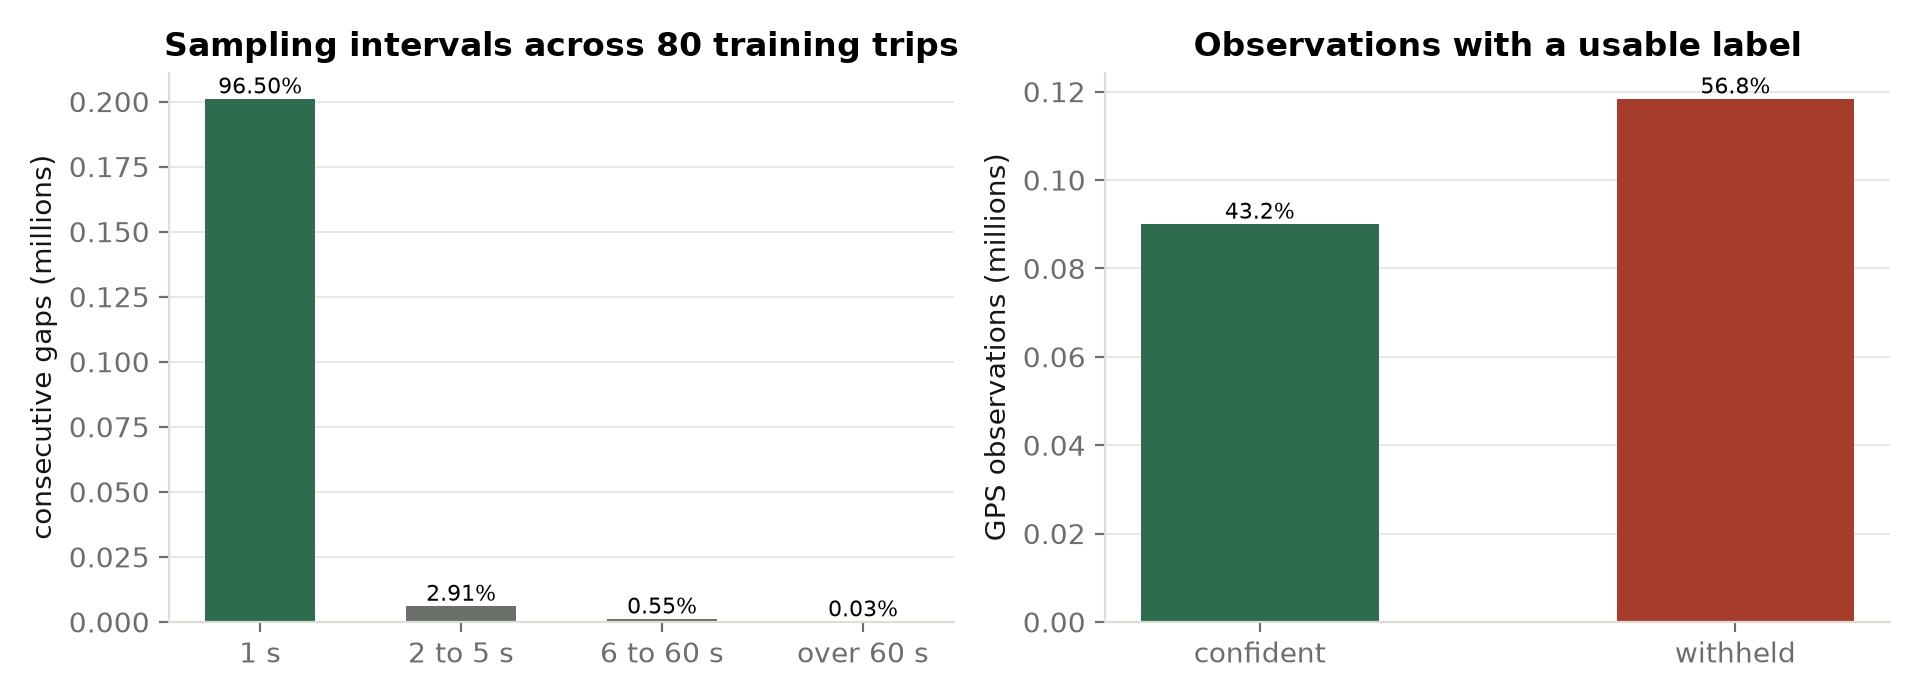
\includegraphics[width=0.94\textwidth]{figures/fig_data_quality.png}
\caption{Left: distribution of consecutive sampling gaps over the 80 training tracks. Right: GPS
observations in the processed training partition that carry a confident label and those the alignment
withheld.}
\label{fig:quality}
\end{figure}
\clearpage

\subsection{Preprocessing}

\begin{enumerate}[leftmargin=1.5em,itemsep=2pt]
\item Parse the four files for a trip. Node and arc identifiers are 0-based row indices, so identity
is positional.
\item Project the trip into a local azimuthal equidistant frame centred on its node extent. All
distances from this point are metres.
\item Generate candidates: every arc within 50 metres of an observation, expanding to 200 metres
when nothing is found, capped at ten candidates ranked by distance.
\item Build features from previous observations only. No future observation and no reference data
enters a feature.
\item Align the reference route to observations with a min-sum forward and backward pass over
ordered route occurrences. The output is a label and a confidence flag per observation.
\item Emit one parquet per trip holding candidate rows, features, a nullable label and an
eligibility flag.
\end{enumerate}

Of 1,304,456 candidate rows across the 80 training trips, 480,258 carried a confident label, or 36.8\%. The remainder were withheld by the alignment rather than guessed. After filtering, 70 of the 80 trips contribute labelled rows; the other 10 produced no confident alignment at all.

\subsection{Features and their justification}

Eighteen features describe each observation and candidate pair, grouped in
Table~\ref{tab:features}. The design rule was that every feature must mean the same thing in every
city: metres, normalised fractions, angles encoded as sines and cosines, and elapsed time. Latitude
and longitude are deliberately excluded.

\begin{table}[H]
\centering
\caption{Feature groups. Every column is scale-free or expressed in metres, so the model transfers
to a city it has never seen.}
\label{tab:features}
\small
\begin{tabular}{@{}p{0.30\textwidth}p{0.30\textwidth}p{0.30\textwidth}@{}}
\toprule
\textbf{Group} & \textbf{What it captures} & \textbf{Why it transfers} \\
\midrule
distance\_m, candidate\_rank & Fit of the observation to the arc & Metres and rank, same meaning anywhere \\
position\_fraction, position\_m, length\_m & Where along the arc the point falls & Normalised and metric \\
road\_sin, road\_cos, heading\_sin, heading\_cos, heading\_difference\_rad & Travel direction against road direction & Sines and cosines avoid the wrap at 0 and 360 \\
movement\_m, dt\_s, speed\_mps, valid\_time\_gap, stationary & Motion between observations & Time based, survives 20 to 149 km/h \\
gaussian\_emission\_20m, log\_emission\_20m & The decoder's emission term & Derived from distance alone \\
\bottomrule
\end{tabular}
\end{table}

\begin{figure}[H]
\centering
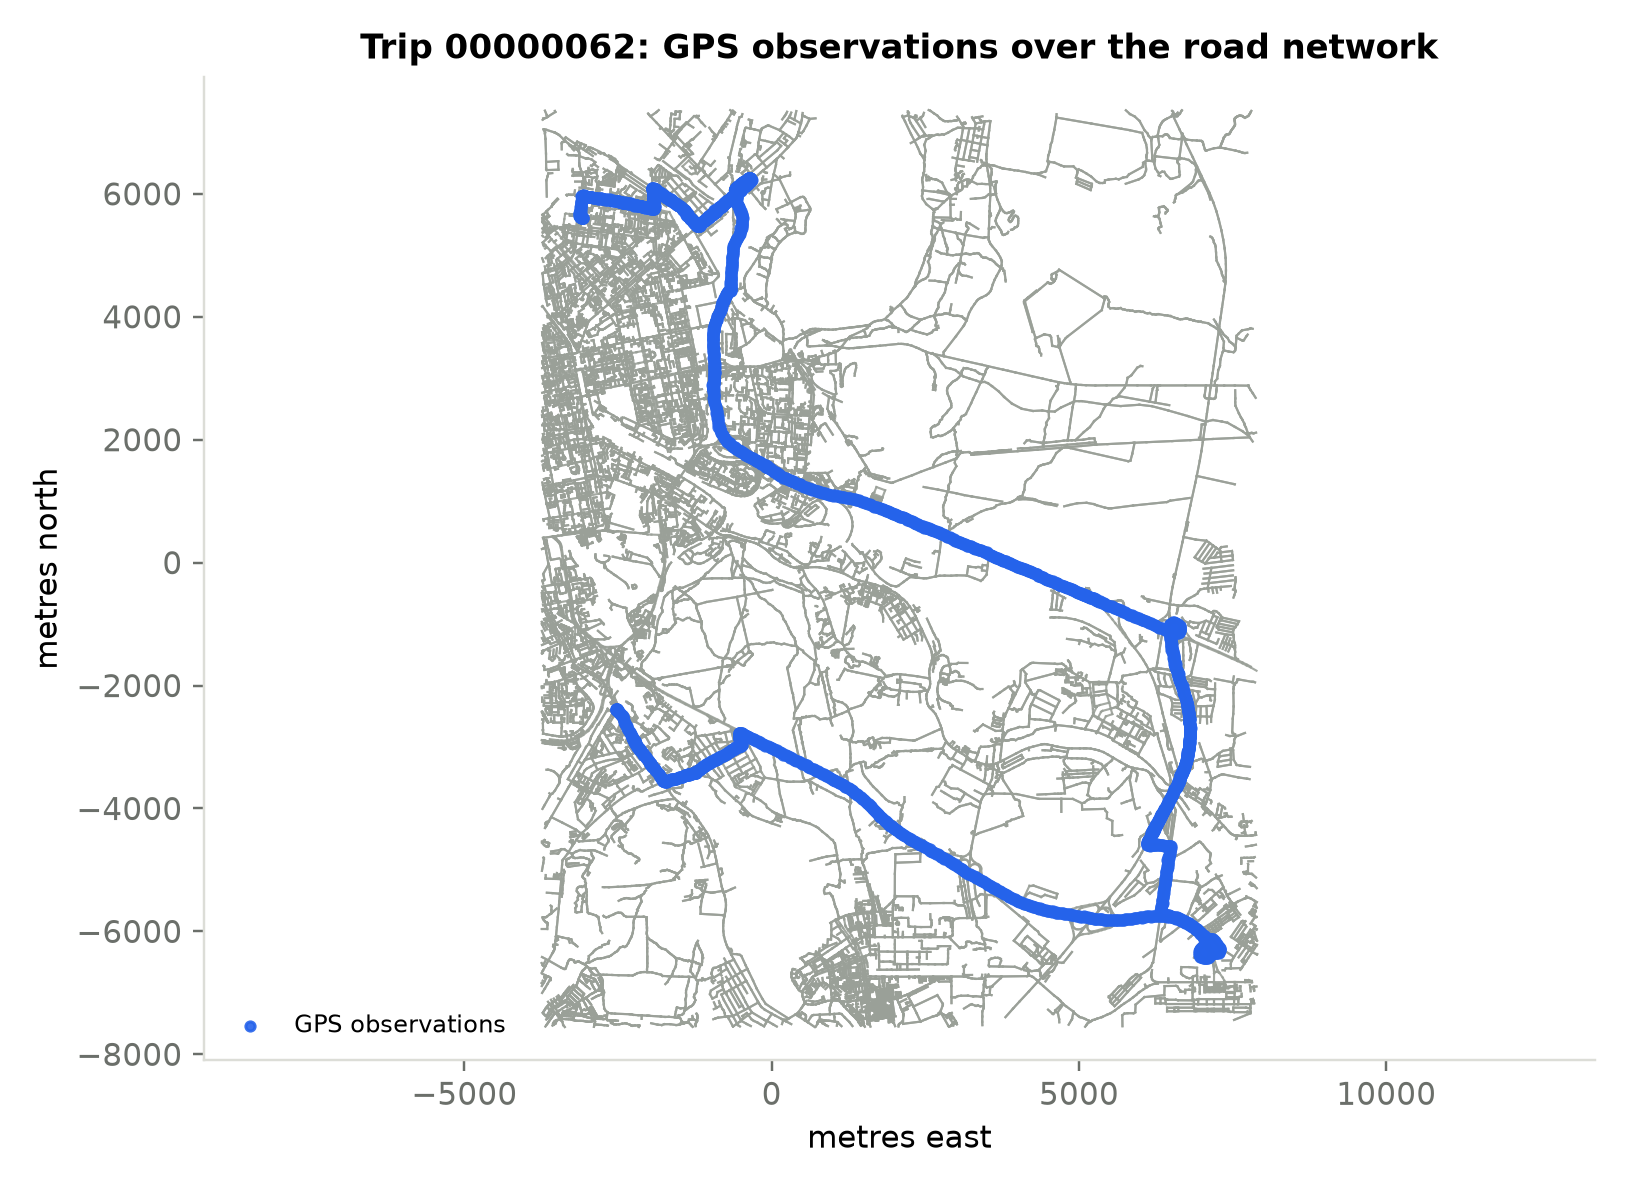
\includegraphics[width=0.7\textwidth]{figures/fig_gps_over_roads.png}
\caption{Trip 00000062 in its local metric frame. Blue marks are GPS observations and grey lines are
the road network. The offset between the trace and the carriageway is the error the model has to
absorb.}
\label{fig:gps}
\end{figure}
\clearpage

\section{Model experimentation and comparison}

Predicting an arc identifier directly is not viable. Arc identifiers are row positions inside one
trip, so the same integer means a different road in another city, and there are thousands of classes
per trip with no relationship between them. The formulation used instead is binary candidate
classification. Each observation contributes several candidate arcs, each pair carries a label
stating whether that arc is the aligned reference arc, and the model learns to score a candidate. The
highest scoring candidate is the classifier-only prediction.

Five model families were trained on the labelled training rows with five-fold grouped
cross-validation, where folds are grouped by trip. Preprocessing sits inside each fold, so imputation
is fitted on training rows only. Table~\ref{tab:comparison} reports the result. Observation-level
Top-1 is measured per GPS point rather than per candidate row, because row accuracy is dominated by
negatives and would flatter a model that rejects everything.

\begin{table}[H]
\centering
\caption{Comparison of the five models. Cross-validation uses five folds grouped by trip and every
student-test score comes from the ten development trips, which were never used for fitting. Route
continuity is measured on the classifier's sequence of best candidates, because the decoder is shared
by all five models; its own continuity is reported in Section~\ref{sec:hmm}. Inference time is the
fastest of three prediction passes over the student-test candidates.}
\label{tab:comparison}
\footnotesize
\resizebox{\textwidth}{!}{%
\begin{tabular}{@{}llp{0.19\textwidth}cccccc@{}}
\toprule
\textbf{Model} & \textbf{Family} & \textbf{Key configuration} & \textbf{CV macro F1}
 & \textbf{Test Top-1} & \textbf{Route continuity} & \textbf{Test macro F1}
 & \textbf{Log loss} & \textbf{Inference (ms)} \\
\midrule
RandomForest & Ensemble & 80 trees, \texttt{min\_samples\_leaf} 2 & 0.848 $\pm$ 0.050 & 82.3\% & 96.9\% & 90.3\% & 0.211 & 270 \\
HistGradientBoosting & Boosting & 200 iterations, \texttt{learning\_rate} 0.1 & 0.845 $\pm$ 0.052 & 81.6\% & 97.2\% & 90.3\% & 0.168 & 263 \\
LogisticRegression & Linear & \texttt{C} 1.0, deprecated penalty & 0.822 $\pm$ 0.041 & 81.1\% & 97.6\% & 87.3\% & 0.234 & 12 \\
GaussianNB & Probabilistic & \texttt{var\_smoothing} 1e-09 & 0.720 $\pm$ 0.025 & 75.3\% & 97.5\% & 74.7\% & 1.094 & 26 \\
DecisionTree & Tree & Gini impurity, \texttt{max\_depth} 18 & 0.821 $\pm$ 0.045 & 78.3\% & 93.5\% & 87.7\% & 1.241 & 11 \\
\bottomrule
\end{tabular}}
\end{table}

The shipped model is \textbf{HistGradientBoosting}.

Top-1 accuracy is the primary metric because the task asks for one road per observation. Macro F1
and log loss describe probability quality, which matters because those probabilities become the
decoder's emissions. Models within 0.010 cross-validated Top-1 of the best were treated as tied and
ranked by log loss. That rule changed no accuracy decision, and it produced a 739 kB artifact instead of the 243 MB forest, which would also exceed repository limits.

Route continuity in the table is the share of consecutive best-candidate arcs that a directed road
path can connect inside the decoder's link limit. It is a property of the candidate ranking, so it can
be measured for every model without running Viterbi, and it separates connectivity failures from
local scoring failures. Inference time excludes candidate generation and metric scoring; the two models
compared in Section~\ref{sec:tuning} were timed the same way.

\subsection{Analysis of each model}
\subsubsection*{RandomForest}
\noindent\textit{Role.} Variance reduction. It handles feature interactions with little tuning and produced the highest raw Top-1 in cross-validation. Its probability estimate is the mean over many trees, which keeps it reasonable though still worse than boosting. It was not shipped because the fitted artifact is 243 MB, beyond repository limits, for half a point of accuracy.

\begin{center}\small\begin{tabular}{@{}ll@{}}\toprule\textbf{Hyperparameter} & \textbf{Initial value} \\ \midrule
n\_estimators & 80 \\
max\_depth & None \\
min\_samples\_leaf & 2 \\
max\_features & sqrt \\
\bottomrule\end{tabular}\end{center}

\noindent\textit{Objective.} Gini impurity averaged over bootstrap samples.

\noindent\textit{Measured.} On the student-testing trips the candidate classifier reached precision 91.1\%, recall 77.8\% and macro F1 90.3\%, with observation-level Top-1 82.3\% and log loss 0.211, and its best-candidate sequence was 96.9\% continuous. Cross-validated macro F1 was 0.848 with a fold standard deviation of 0.050, cross-validated Top-1 was 73.2\%, the mean fit took 52.2 seconds per fold, and inference took 270 milliseconds.

\noindent\textit{Strengths and limitations.} Strengths: the best raw Top-1 on the student-test partition, feature interactions handled without scaling, and a probability that is an average over eighty trees. Limitations: a 243 MB artifact, the slowest scoring path of the five and probabilities that are good but not as sharp as boosting.

\noindent\textit{Overfitting check.} Cross-validated Top-1 was 73.2\% and student-test Top-1 was 82.3\%, a gap of 9.1 percentage points. No sign of overfitting: the student-test score sits within a point of the cross-validated score and the fold spread is moderate.

\subsubsection*{HistGradientBoosting}
\noindent\textit{Role.} Sequential correction. It matches the forest on macro F1 and beats it on log loss, which matters because those probabilities become the decoder's emissions. It also fits roughly five times faster and ships as a 740 kB artifact. This is the model behind the deployed system.

\begin{center}\small\begin{tabular}{@{}ll@{}}\toprule\textbf{Hyperparameter} & \textbf{Initial value} \\ \midrule
max\_iter & 200 \\
learning\_rate & 0.1 \\
max\_leaf\_nodes & 31 \\
min\_samples\_leaf & 20 \\
l2\_regularization & 0.0 \\
\bottomrule\end{tabular}\end{center}

\noindent\textit{Objective.} binary log loss, minimised stagewise with histogram splits.

\noindent\textit{Measured.} On the student-testing trips the candidate classifier reached precision 90.6\%, recall 78.2\% and macro F1 90.3\%, with observation-level Top-1 81.6\% and log loss 0.168, and its best-candidate sequence was 97.2\% continuous. Cross-validated macro F1 was 0.845 with a fold standard deviation of 0.052, cross-validated Top-1 was 72.7\%, the mean fit took 9.1 seconds per fold, and inference took 263 milliseconds.

\noindent\textit{Strengths and limitations.} Strengths: the best log loss of the five, competitive Top-1 and macro F1, a 740 kB artifact and fast scoring. Limitations: it needs careful early-stopping and regularisation settings, and its probability output is only as good as the candidate set it scores.

\noindent\textit{Overfitting check.} Cross-validated Top-1 was 72.7\% and student-test Top-1 was 81.6\%, a gap of 8.9 percentage points. No sign of overfitting: the student-test score is slightly above the cross-validated score, and the log loss improves in the same direction.

\subsubsection*{LogisticRegression}
\noindent\textit{Role.} Linear baseline. It establishes how much signal is available from a weighted sum of the features and trains in about two seconds. It holds up better than expected, which says the features carry useful information and the problem is not purely interaction driven. Its limit is that a linear boundary cannot express thresholds such as a distance cut-off.

\begin{center}\small\begin{tabular}{@{}ll@{}}\toprule\textbf{Hyperparameter} & \textbf{Initial value} \\ \midrule
C & 1.0 \\
max\_iter & 1000 \\
solver & lbfgs \\
penalty & deprecated \\
\bottomrule\end{tabular}\end{center}

\noindent\textit{Objective.} binary cross entropy (log loss), minimised by L-BFGS.

\noindent\textit{Measured.} On the student-testing trips the candidate classifier reached precision 81.9\%, recall 76.7\% and macro F1 87.3\%, with observation-level Top-1 81.1\% and log loss 0.234, and its best-candidate sequence was 97.6\% continuous. Cross-validated macro F1 was 0.822 with a fold standard deviation of 0.041, cross-validated Top-1 was 72.7\%, the mean fit took 2.4 seconds per fold, and inference took 12 milliseconds.

\noindent\textit{Strengths and limitations.} Strengths: a stable linear decision surface, honest probabilities and three seconds to train, which makes it a useful reference point. Limitations: it cannot represent a rule such as a hard distance cut-off without an explicit interaction term, and it underfits the curved decision boundary that the features describe.

\noindent\textit{Overfitting check.} Cross-validated Top-1 was 72.7\% and student-test Top-1 was 81.1\%, a gap of 8.5 percentage points. The gap is small and the linear boundary transfers; the shortfall is capacity, not variance.

\subsubsection*{GaussianNB}
\noindent\textit{Role.} Probabilistic floor. It is cheap, needs no tuning, and its independence assumption is plainly wrong here because distance and heading are correlated. The measured log loss confirms that: it is the worst of the five while accuracy stays respectable, which is what an over-confident independence assumption looks like.

\begin{center}\small\begin{tabular}{@{}ll@{}}\toprule\textbf{Hyperparameter} & \textbf{Initial value} \\ \midrule
var\_smoothing & 1e-09 \\
\bottomrule\end{tabular}\end{center}

\noindent\textit{Objective.} maximum likelihood under a Gaussian assumption; no iterative loss.

\noindent\textit{Measured.} On the student-testing trips the candidate classifier reached precision 48.8\%, recall 86.9\% and macro F1 74.7\%, with observation-level Top-1 75.3\% and log loss 1.094, and its best-candidate sequence was 97.5\% continuous. Cross-validated macro F1 was 0.720 with a fold standard deviation of 0.025, cross-validated Top-1 was 69.8\%, the mean fit took 0.8 seconds per fold, and inference took 26 milliseconds.

\noindent\textit{Strengths and limitations.} Strengths: no tuning, a fraction of a second to fit, and a closed-form probability. Limitations: it treats every feature as independent, so two features that say the same thing are counted twice, and its probabilities are not calibrated.

\noindent\textit{Overfitting check.} Cross-validated Top-1 was 69.8\% and student-test Top-1 was 75.3\%, a gap of 5.5 percentage points. The gap is small, but the model is last on every probability metric, which is underfitting: the independence assumption caps how well it can rank candidates.

\subsubsection*{DecisionTree}
\noindent\textit{Role.} Threshold reader. It tests whether axis-aligned rules are enough and produces rules a person can inspect. The log loss shows severe over-confidence: leaf probabilities collapse to zero and one, so the loss is an order of magnitude worse than the ensembles.

\begin{center}\small\begin{tabular}{@{}ll@{}}\toprule\textbf{Hyperparameter} & \textbf{Initial value} \\ \midrule
max\_depth & 18 \\
criterion & gini \\
min\_samples\_split & 2 \\
min\_samples\_leaf & 1 \\
\bottomrule\end{tabular}\end{center}

\noindent\textit{Objective.} Gini impurity for the split criterion.

\noindent\textit{Measured.} On the student-testing trips the candidate classifier reached precision 82.1\%, recall 77.7\% and macro F1 87.7\%, with observation-level Top-1 78.3\% and log loss 1.241, and its best-candidate sequence was 93.5\% continuous. Cross-validated macro F1 was 0.821 with a fold standard deviation of 0.045, cross-validated Top-1 was 68.8\%, the mean fit took 8.9 seconds per fold, and inference took 11 milliseconds.

\noindent\textit{Strengths and limitations.} Strengths: interpretable axis-aligned rules and no scaling requirement. Limitations: a single tree is a high-variance estimator, and its leaf probabilities collapse towards zero and one, which is why its log loss is unusable even where its argmax is fine.

\noindent\textit{Overfitting check.} Cross-validated Top-1 was 68.8\% and student-test Top-1 was 78.3\%, a gap of 9.5 percentage points. Accuracy generalises while the log loss does not, so the tree overfits in probability space even where its argmax is acceptable.


\subsection{Candidate-level confusion matrix}

The table above aggregates, and an aggregate can hide where the errors sit. Figure~\ref{fig:confusion}
breaks the shipped model's decisions on the student-test candidates into the four cells of a confusion
matrix, using the default 0.5 threshold. There are 54,596 labelled candidate rows: 7,929 true positives, 820 false positives, 2,212 false negatives and 43,635 true negatives. That gives candidate precision 90.6\%, recall 78.2\% and F1 83.9\%.

The asymmetry is in the useful direction. A false positive only hurts when it outranks the true
candidate, and with only 1.50\% of rows falling there, most of them never reach the top of a ranking. A false negative
is the more expensive error. The reference arc was rejected outright, so the decoder has to recover
from a neighbour and the observation can only be correct by luck. The counts also show why the hard
labels are a diagnostic rather than the objective. The decoder never reads a 0/1 decision, it reads
the probability itself, which is why selection was settled on log loss once Top-1 tied.

\begin{figure}[H]
\centering
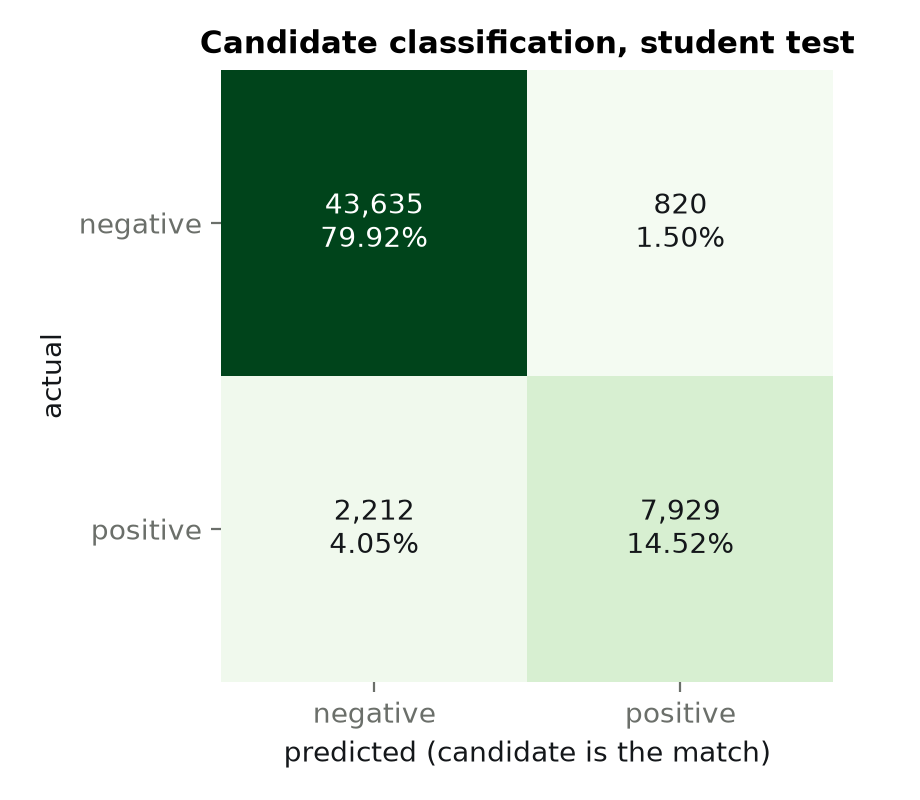
\includegraphics[width=0.5\textwidth]{figures/fig_confusion_matrix.png}
\caption{Candidate-level confusion matrix for the shipped model on the student-test partition. Cell
labels give the row count and the share of all candidate rows.}
\label{fig:confusion}
\end{figure}

\subsection{Final evaluation on the reserved partition}

The ten reserved trips were supplied after the model, the decoder and every hyperparameter had been
fixed. They were used for scoring only, and no decision in this report depends on them.

\begin{table}[H]
\centering
\caption{Reserved evaluator partition. Every trip was run through the deployed API, with the reference
route used only after the prediction existed.}
\label{tab:evaluator}
\small
\begin{tabular}{@{}lccccc@{}}
\toprule
\textbf{Trip} & \textbf{Evaluable} & \textbf{Classifier Top-1} & \textbf{Decoded accuracy}
 & \textbf{Continuity} & \textbf{Candidate miss} \\
\midrule
00000015 & 3832 & 24.1\% & 46.1\% & 100.0\% & 2.6\% \\
00000017 & 360 & 94.4\% & 98.1\% & 100.0\% & 0.6\% \\
00000023 & 343 & 98.5\% & 99.4\% & 100.0\% & 0.3\% \\
00000030 & 210 & 77.6\% & 88.6\% & 100.0\% & 2.4\% \\
00000049 & 1948 & 97.5\% & 99.5\% & 100.0\% & 0.0\% \\
00000059 & 372 & 96.2\% & 98.1\% & 100.0\% & 0.0\% \\
00000067 & 627 & 71.3\% & 90.6\% & 100.0\% & 0.0\% \\
00000073 & 540 & 96.7\% & 99.4\% & 100.0\% & 0.0\% \\
00000087 & 835 & 97.2\% & 99.6\% & 100.0\% & 0.0\% \\
00000094 & 1397 & 65.1\% & 79.3\% & 100.0\% & 0.3\% \\
\bottomrule
\end{tabular}
\end{table}

Across the ten reserved trips the decoded accuracy averaged \textbf{89.9\%}, between 46.1 and 99.6\%. The classifier alone averaged 81.9\%, so decoding was worth \textbf{8.0 percentage points} on trips the model had never seen.

Trip 00000015 is the outlier at 46.1\%. Its road extract is sparse, 3,225 arcs across a 53 kilometre drive, so long
stretches repeat a single arc and only 3,832 of 6,854 observations produced a confident reference
alignment. The result is reported as measured. Figure~\ref{fig:evaluator} shows the same comparison
trip by trip.

\begin{figure}[H]
\centering
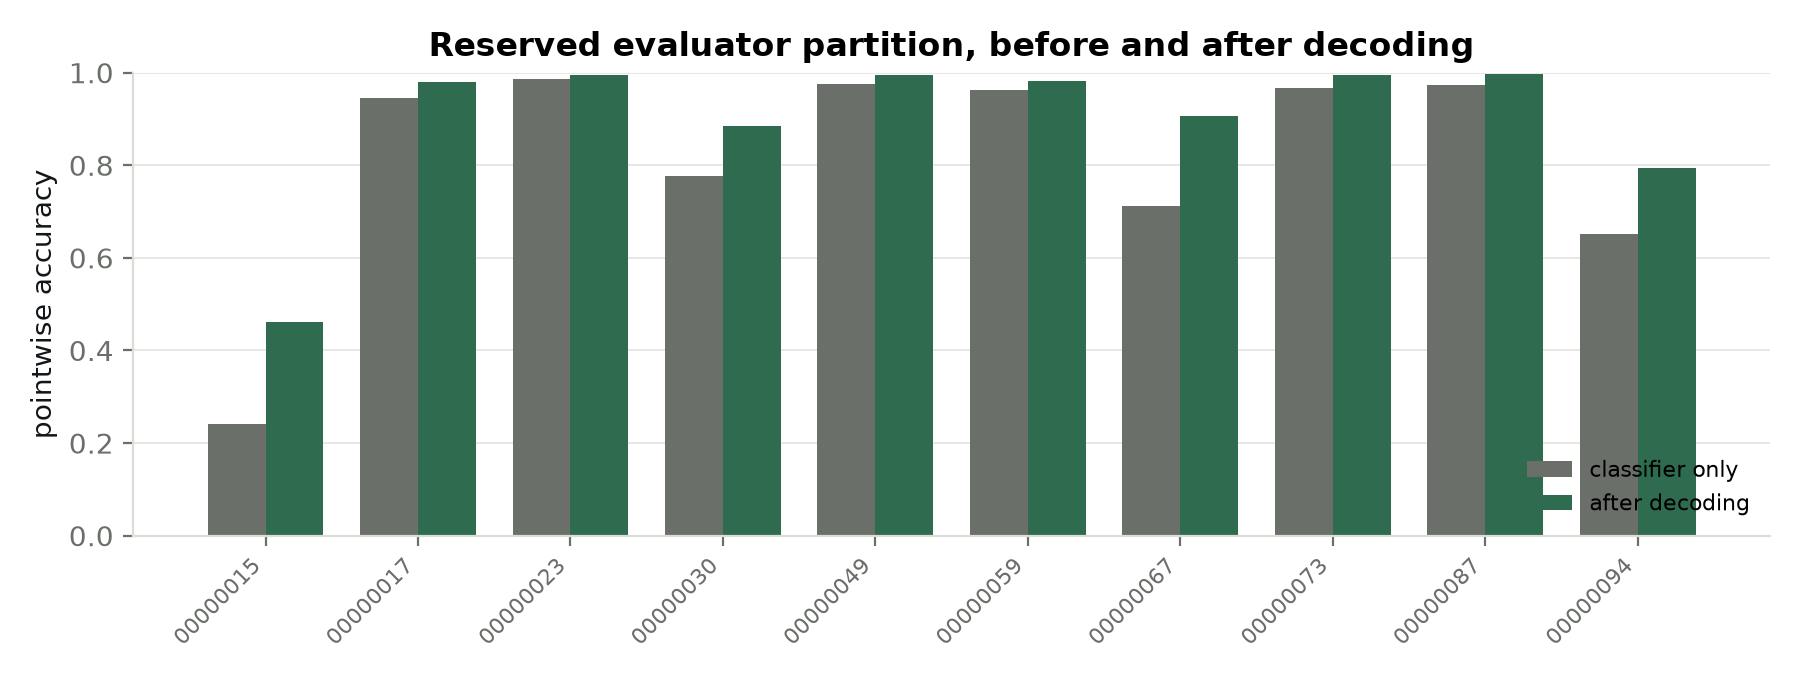
\includegraphics[width=0.94\textwidth]{figures/fig_evaluator_trips.png}
\caption{Reserved evaluator partition, classifier Top-1 against decoded pointwise accuracy. Every bar
pair is one trip; the decoder is above the classifier on all ten.}
\label{fig:evaluator}
\end{figure}

\begin{figure}[H]
\centering
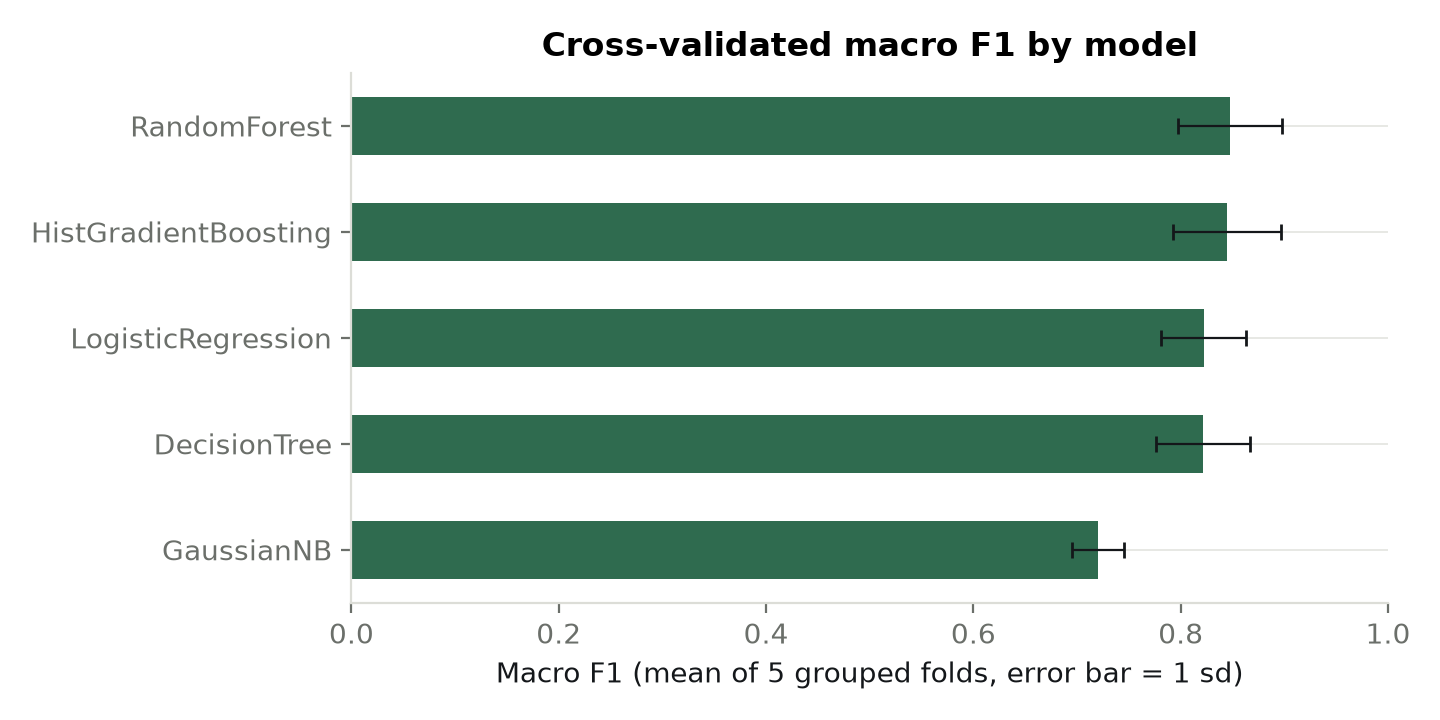
\includegraphics[width=0.84\textwidth]{figures/fig_cv_macro_f1.png}
\caption{Cross-validated macro F1 for each model, with one standard deviation across the five grouped
folds.}
\label{fig:cv}
\end{figure}

\begin{figure}[H]
\centering
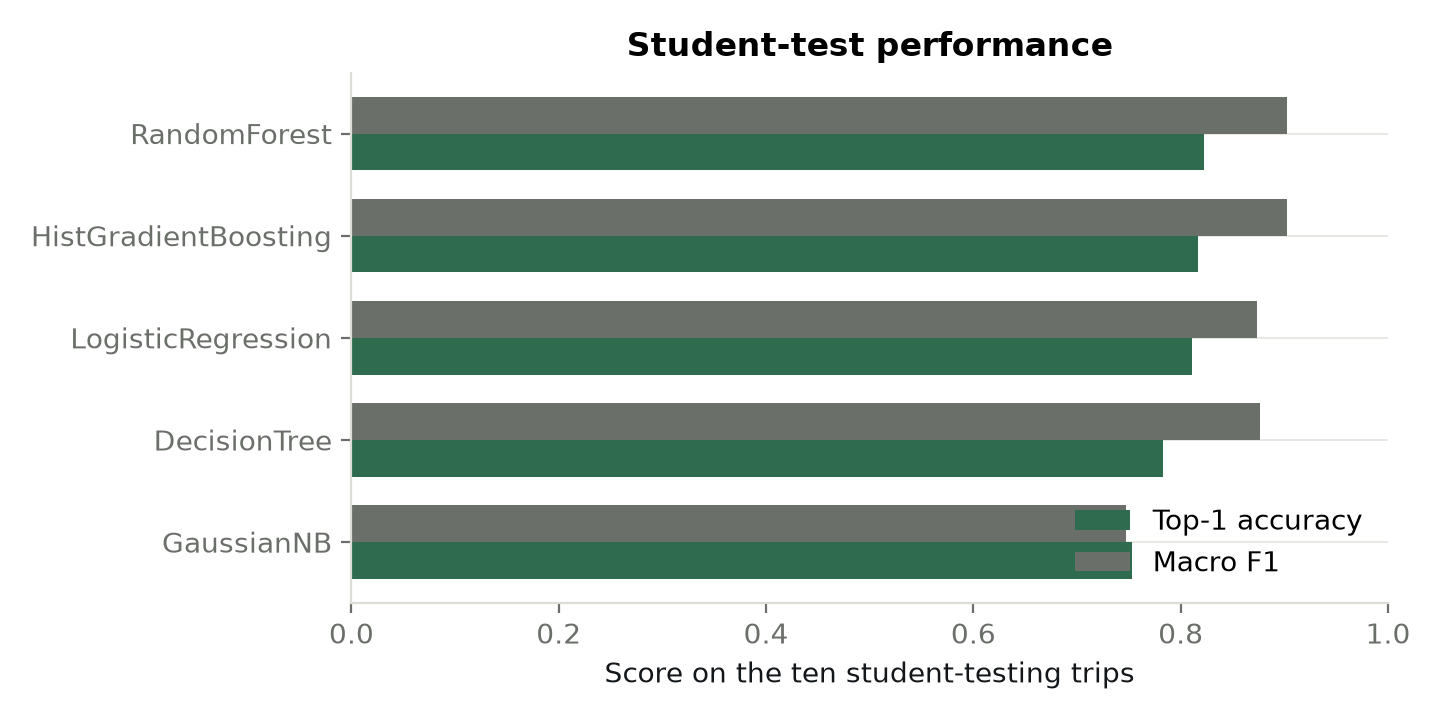
\includegraphics[width=0.84\textwidth]{figures/fig_test_top1_macro_f1.png}
\caption{Student-test Top-1 accuracy and macro F1 for the same five models.}
\label{fig:test}
\end{figure}

\begin{figure}[H]
\centering
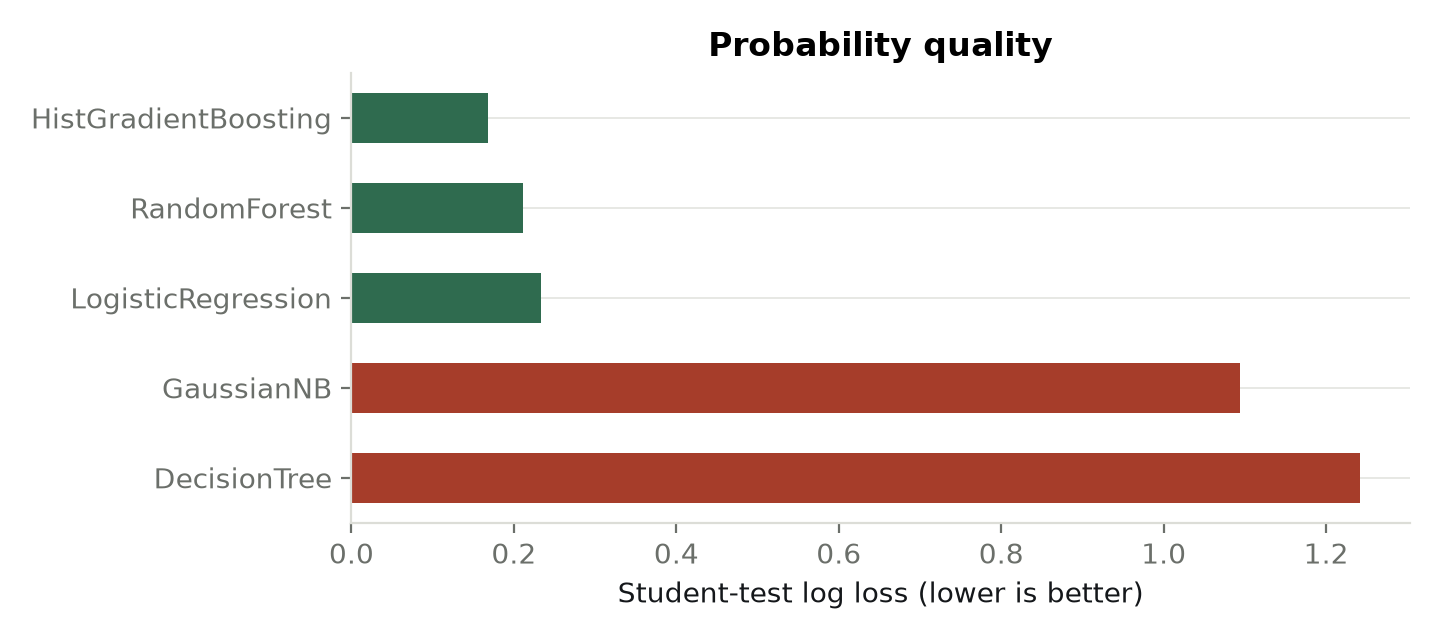
\includegraphics[width=0.78\textwidth]{figures/fig_log_loss.png}
\caption{Student-test log loss. The single decision tree is badly over-confident, which is why its
probabilities are unusable as decoder emissions.}
\label{fig:logloss}
\end{figure}
\clearpage
\section{Bayesian hyperparameter optimisation}
\label{sec:tuning}
The selected algorithm was tuned with Optuna's Tree-structured Parzen Estimator, a
Bayesian sampler that models which regions of the search space produce good trials instead of
sampling uniformly. The objective combined observation-level Top-1 and macro F1, averaged over three
folds grouped by trip, so tuning could not benefit from a lucky split.

\begin{table}[H]
\centering
\caption{Bayesian search settings and outcome.}
\label{tab:tuning}
\begin{tabular}{@{}p{0.30\textwidth}p{0.63\textwidth}@{}}
\toprule
\textbf{Item} & \textbf{Value} \\
\midrule
Sampler & TPE, seed 42 \\
Trials & 10 \\
Search space & \texttt{max\_iter} 100 to 350, \texttt{learning\_rate} 0.03 to 0.3 (log),
\texttt{max\_leaf\_nodes} 15 to 63, \texttt{min\_samples\_leaf} 10 to 60,
\texttt{l2\_regularization} \(10^{-4}\) to 10 (log) \\
Objective & \(0.7 \times\) Top-1 \(+\) \(0.3 \times\) macro F1 over three grouped folds \\
Best objective & 0.7651 \\
Tuned student-test Top-1 & 81.5\% \\
Untuned student-test Top-1 & 81.6\% \\
\bottomrule
\end{tabular}
\end{table}

\begin{table}[H]
\centering
\caption{Best configuration returned by the search.}
\label{tab:bestparams}
\begin{tabular}{@{}ll@{}}
\toprule
\textbf{Hyperparameter} & \textbf{Best value} \\
\midrule
max\_iter & 100 \\
learning\_rate & 0.034293 \\
max\_leaf\_nodes & 57 \\
min\_samples\_leaf & 40 \\
l2\_regularization & 0.347027 \\
\bottomrule
\end{tabular}
\end{table}

Table~\ref{tab:tuned} repeats the comparison on the same folds and the same student-test rows, so the
only difference between the two rows is the hyperparameter configuration.

\begin{table}[H]
\centering
\caption{Tuned against untuned model on identical folds and identical student-test rows. Inference time
is the fastest of three prediction passes over the student-test candidates.}
\label{tab:tuned}
\small
\resizebox{\textwidth}{!}{%
\begin{tabular}{@{}lccccc@{}}
\toprule
\textbf{Variant} & \textbf{CV macro F1} & \textbf{Test macro F1} & \textbf{Test Top-1}
 & \textbf{Log loss} & \textbf{Inference (ms)} \\
\midrule
untuned (HistGradientBoosting) & 0.845 $\pm$ 0.046 & 90.3\% & 81.6\% & 0.168 & 232 \\
tuned (Optuna TPE) & 0.847 $\pm$ 0.047 & 90.2\% & 81.5\% & 0.170 & 174 \\
\bottomrule
\end{tabular}}
\end{table}

The tuned configuration did not improve the model. Cross-validated macro F1 rose slightly, while
student-test macro F1 and student-test Top-1 both fell and log loss moved the wrong way. The one clear
gain is inference time, and it comes from the search choosing a smaller number of boosting iterations
than the default, not from a better model. On a dataset this size the metric movements sit inside the
fold noise, so a model that is equal on accuracy, slightly worse on calibration and faster only because
it is smaller has no argument to replace the one already in the report. The tuned pipeline was
therefore not adopted.

The search still did its job. It probed a wide region and the defaults won, which says the default
configuration sat near the optimum of this space. The full trial
record, including every sampled configuration and its objective, is kept in
\texttt{results/optuna\_trials.csv}.

\begin{figure}[H]
\centering
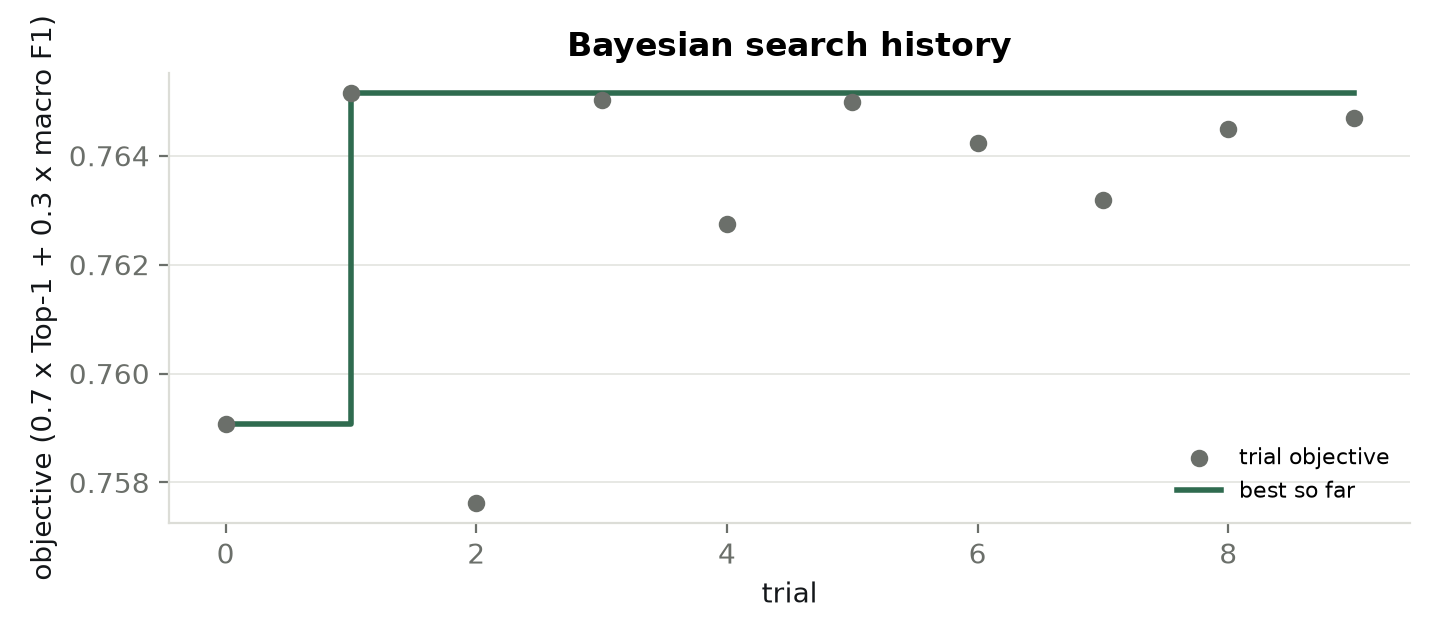
\includegraphics[width=0.78\textwidth]{figures/fig_optuna_history.png}
\caption{Objective value for each Bayesian trial. The step line is the best value seen so far; later
trials did not improve it.}
\label{fig:optuna}
\end{figure}

\section{HMM and Viterbi route reconstruction}
\label{sec:hmm}

A classifier scores candidates independently, so consecutive observations can land on arcs that no
vehicle could drive between. The decoder resolves this by scoring whole sequences rather than single
observations.

\begin{table}[H]
\centering
\caption{Decoder design.}
\label{tab:hmm}
\small
\begin{tabular}{@{}p{0.22\textwidth}p{0.70\textwidth}@{}}
\toprule
\textbf{Component} & \textbf{Choice} \\
\midrule
Hidden states & The candidate arcs available at each observation, each carrying its projection
fraction along the arc. \\
\midrule
Emission & The classifier's positive-class probability, clipped, normalised across the candidates of
that observation, then logged. A binary probability is not a distribution over candidates, so
normalisation is required before states can be compared. \\
\midrule
Transition & Directed road distance from the previous candidate to the next, measured with a bounded
Dijkstra over the sparse adjacency matrix. The score penalises the difference between road distance
and GPS displacement, backwards movement, and speeds above 50 metres per second. \\
\midrule
Missing candidates & Observations with no candidate inside the radius are absent from the grid. The
transition then spans the real time gap, and the response reports how many observations were
affected. \\
\midrule
Disconnected pairs & When no road link exists within 400 metres the pair receives a heavy finite
penalty scaled by straight-line distance, so one unreachable pair cannot make a whole trip
undecodable. Pairs beyond two kilometres are set to negative infinity. \\
\bottomrule
\end{tabular}
\end{table}

After Viterbi has chosen an arc per observation, a reconstruction pass turns that sequence into
travelled portions of road. Each chosen arc keeps a start and end offset along its length, so the
drawn route follows the part of the arc the vehicle used rather than hopping between arc endpoints.
Pieces split only where the road network cannot connect them, which is where the route pieces in the
figures come from.

\subsection{Classifier alone against classifier plus decoder}

The same observations, the same alignment and the same scoring rule were used for both paths, so the
only difference is the decoder.

\begin{table}[H]
\centering
\caption{Pointwise accuracy with and without sequential decoding, on development trips.}
\label{tab:decoder}
\small
\resizebox{\textwidth}{!}{%
\begin{tabular}{@{}lccccc@{}}
\toprule
\textbf{Trip} & \textbf{Evaluable} & \textbf{Classifier Top-1} & \textbf{Decoded}
 & \textbf{Classifier continuity} & \textbf{Decoded continuity} \\
\midrule
00000000 & 2099 & 95.2\% & 96.3\% & 98.2\% & 99.9\% \\
00000007 & 929 & 97.2\% & 99.0\% & 99.6\% & 100.0\% \\
00000009 & 217 & 89.9\% & 94.0\% & 99.5\% & 100.0\% \\
00000052 & 150 & 99.3\% & 100.0\% & 94.6\% & 100.0\% \\
00000091 & 398 & 73.9\% & 79.1\% & 96.2\% & 100.0\% \\
\bottomrule
\end{tabular}}
\end{table}

Decoding improved pointwise accuracy on every trip measured, by between 0.7 and 5.3 percentage points. The largest gains appear where the classifier is weakest, which
is the expected behaviour. When local evidence is ambiguous, connectivity carries the decision.

\subsection{Route-level agreement with the reference sequence}

Pointwise accuracy scores one observation at a time, so it cannot see whether the arcs come out in a
driveable order. The sequence measure does. Each trip's prediction is reduced to its ordered list of
distinct arcs, that list is turned into the set of consecutive arc pairs it contains, and the set is
compared with the pairs in the reference route. Precision is the share of predicted pairs that occur
in the reference, recall is the share of reference pairs that were predicted, and the F1 of the two is
the route-level score.

\begin{table}[H]
\centering
\caption{Route-level agreement on the student-test trips. Pairs are consecutive arcs in the
deduplicated sequence, so a repeated arc is counted once.}
\label{tab:sequence}
\footnotesize
\resizebox{\textwidth}{!}{%
\begin{tabular}{@{}lccccccc@{}}
\toprule
\textbf{Trip} & \textbf{Reference arcs} & \textbf{Classifier P} & \textbf{Classifier R}
 & \textbf{Classifier F1} & \textbf{Decoded P} & \textbf{Decoded R} & \textbf{Decoded F1} \\
\midrule
00000000 & 145 & 48.0\% & 74.3\% & 58.3\% & 64.7\% & 82.6\% & 72.6\% \\
00000007 & 91 & 44.8\% & 71.1\% & 54.9\% & 64.2\% & 85.6\% & 73.3\% \\
00000009 & 74 & 5.0\% & 30.1\% & 8.6\% & 7.9\% & 39.7\% & 13.2\% \\
00000040 & 223 & 41.6\% & 67.1\% & 51.4\% & 58.7\% & 82.4\% & 68.5\% \\
00000052 & 38 & 32.0\% & 64.9\% & 42.9\% & 34.2\% & 70.3\% & 46.0\% \\
00000056 & 299 & 15.8\% & 48.3\% & 23.8\% & 20.6\% & 63.8\% & 31.1\% \\
00000065 & 61 & 16.6\% & 40.0\% & 23.4\% & 34.1\% & 71.7\% & 46.2\% \\
00000077 & 162 & 9.3\% & 25.5\% & 13.6\% & 29.2\% & 58.4\% & 38.9\% \\
00000091 & 80 & 13.5\% & 38.0\% & 19.9\% & 23.6\% & 58.2\% & 33.6\% \\
\midrule Mean & -- & 25.2\% & 51.0\% & 33.0\% & 37.5\% & 68.1\% & 47.1\% \\
\bottomrule
\end{tabular}}
\end{table}

The averages tell the same story as the pointwise table. Transition precision rises from 25.2\% to 37.5\% and recall rises from 51.0\% to 68.1\%, which lifts transition F1 from 33.0\% to 47.1\%. The decoded route is closer to the reference on 9 of 9 trips.

The gains are uneven, and the unevenness is informative. The smallest gain is on trip 00000052, about 3 points of F1, a short trip where the classifier was already close to the reference
order and there was little left to repair. The largest gain is on trip 00000077, where the classifier jumps between arcs and decoding lifts F1 by about 25 points.

The weakest prediction is trip 00000009, where decoded F1 is still 13.2\%. The classifier names 437 distinct arcs on that trip against a reference of 74, so the decoded sequence necessarily contains transitions the reference does not have.
The predicted sequence is far longer than the reference, and no transition score can remove arcs that
the classifier keeps choosing.

Decoding did not hurt a single trip, but there are two cases where it cannot help much. The first is
when the reference arc is missing from the candidate set at a radius. No transition score can vote for
a road that was never generated, so recall is capped before the decoder runs. The second is a sparse
extract where one arc covers several observations. Distinct-arc scoring then has very few pairs to
match, and the trip scores low however good the local match is. Both are candidate-generation limits,
not Viterbi limits, and the first is exactly what the candidate miss rate column in
Table~\ref{tab:evaluator} measures.

\begin{figure}[H]
\centering
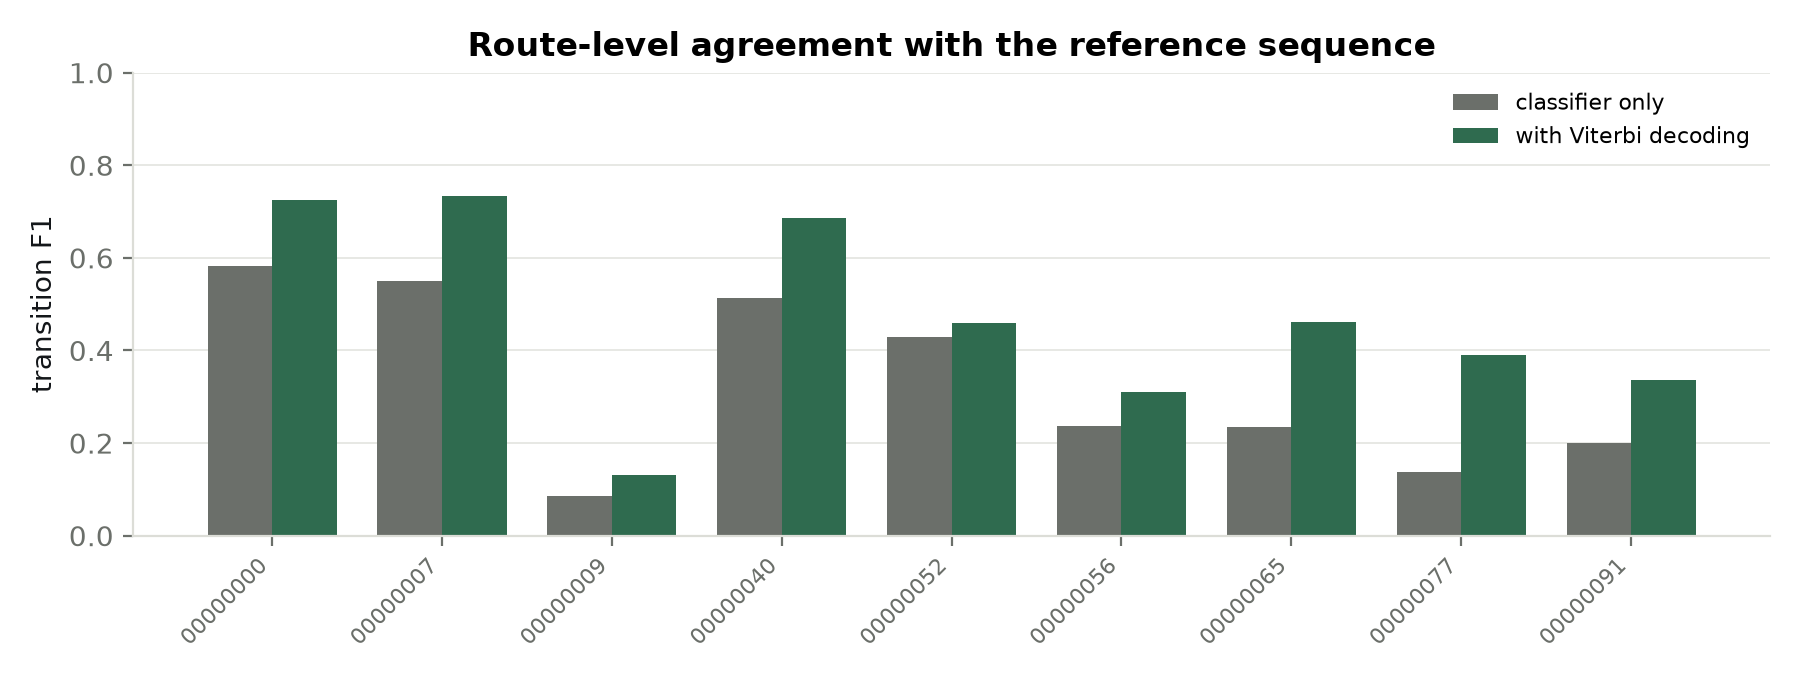
\includegraphics[width=0.98\textwidth]{figures/fig_sequence_f1.png}
\caption{Route-level transition F1 for each student-test trip, classifier only against Viterbi
decoding.}
\label{fig:sequence}
\end{figure}
\clearpage

\section{Geographical visualisation with Folium}

Maps are produced by the map module in \texttt{src/visualization} from live data, and by the report
renderer in \texttt{tools} for the evidence shown here. The evaluator interface renders GPS
observations, the relevant road context and the predicted route. The reference route appears only in
report maps built from training or student-testing trips, never in the interface.

\begin{figure}[H]
\centering
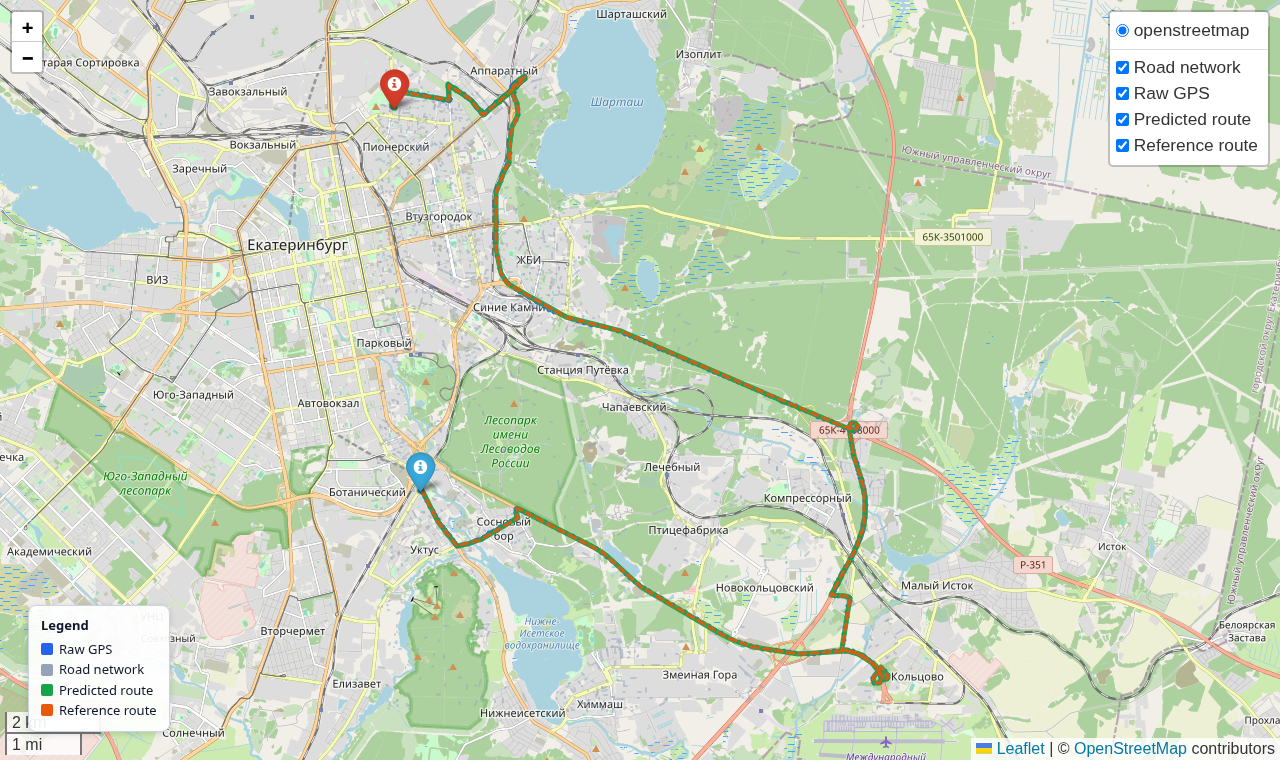
\includegraphics[width=0.98\textwidth]{figures/folium_trip_00000062_layers.png}
\caption{Trip 00000062, Yekaterinburg, with every layer the report tool draws. Grey lines are the road
network, blue marks the raw GPS observations, green is the route predicted by the shipped pipeline and
dashed orange is the reference route. The prediction follows the reference for most of the drive; the
reference is dashed and drawn on top so both stay visible where they overlap. Generated by
\texttt{tools/render\_predicted\_trip\_map.py}, and the interactive HTML with working layer controls is
committed at \texttt{results/maps/trip\_00000062\_layers.html}.}
\label{fig:folium}
\end{figure}

\section{API, UI and deployment}

Laptop 1 runs the FastAPI backend and holds the model, the decoder and the reference routes. Laptop
2 runs the Streamlit interface and reaches the backend over the local network. Ground truth never
crosses that link. The response contract has no field for the reference route.

The service runs in one of two modes. In trained mode it builds candidates, scores them, decodes a
route and then scores that route against the reference, so the response carries accuracy, Top-1,
continuity and candidate miss rate. In evaluator mode it reads candidate probabilities that were
computed ahead of time and never opens a reference route at all, so the response carries only
geometry, continuity and runtime. The interface screenshot in Figure~\ref{fig:ui} comes from an
evaluator-mode run, which is why its readout shows a single metric, and the request log in
Figure~\ref{fig:apilog} comes from a trained-mode run, which is why it carries an accuracy. Nothing
is hidden. The health endpoint names the mode, and the response omits what was not computed.

The pair was exercised over the shared network with the API on Laptop 1 at \texttt{10.30.201.178:8000}
and the interface on Laptop 2. A prediction for trip 00000023 returned in 1,196 milliseconds,
measured at the interface.

\begin{table}[H]
\centering
\caption{Public endpoints.}
\label{tab:api}
\small
\begin{tabular}{@{}p{0.20\textwidth}p{0.72\textwidth}@{}}
\toprule
\textbf{Endpoint} & \textbf{Purpose} \\
\midrule
\texttt{GET /health} & Liveness, trip count and the loaded model name. \\
\texttt{GET /trips} & Trip identifiers discovered from the server directory. Nothing is hardcoded,
so the reserved partition appears without a code change. \\
\texttt{POST /predict} & Runs candidates, features, scoring and decoding, then scores the result
against the reference route held on the server. \\
\bottomrule
\end{tabular}
\end{table}

\begin{figure}[H]
\centering
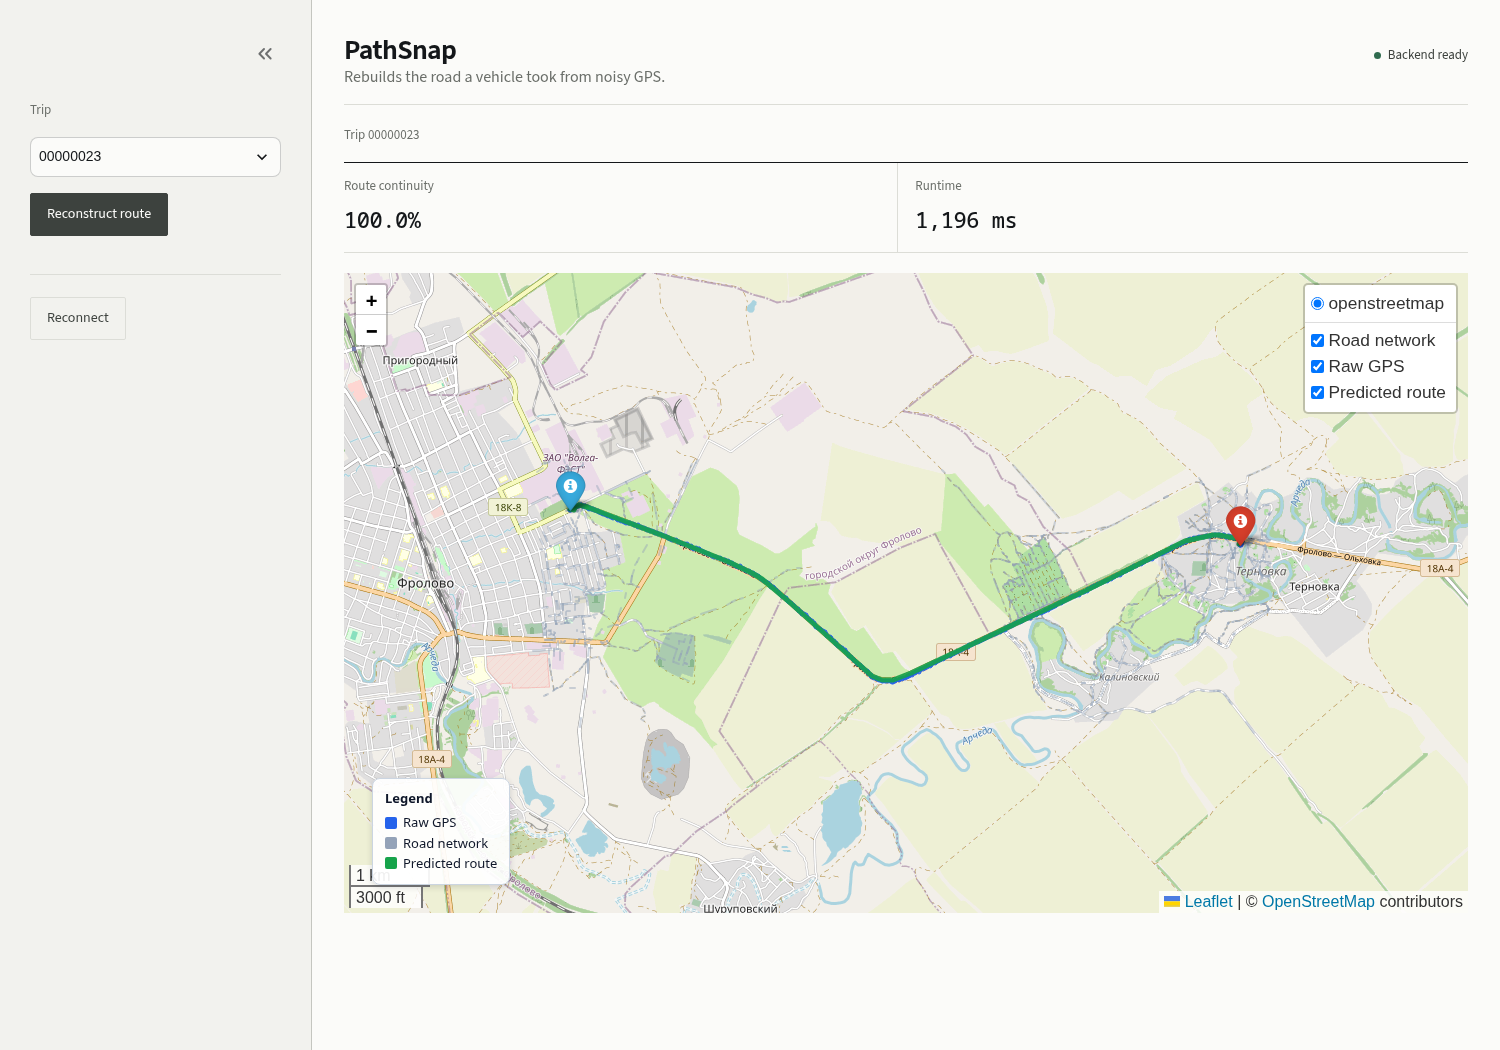
\includegraphics[width=0.99\textwidth]{figures/ui_lan_prediction.png}
\caption{The interface on Laptop 2, served by the backend on Laptop 1 over the shared network. The ten
reserved trips are discovered from the server, so no code changed when the evaluator data arrived.
Trip 00000023 was selected and its route drawn in 1,196 milliseconds. The evaluator mode reports
continuity and runtime only, as described above.}
\label{fig:ui}
\end{figure}

\begin{figure}[H]
\centering
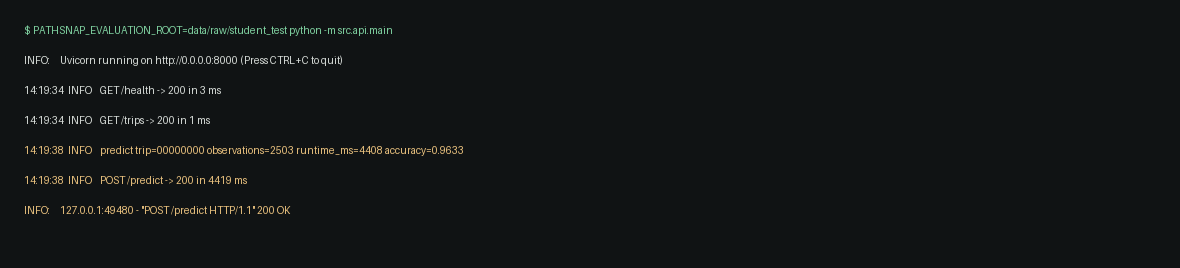
\includegraphics[width=0.98\textwidth]{figures/api_request_log.png}
\caption{Request log on Laptop 1 during a trained-mode run, captured on the machine receiving the
requests. The server answers \texttt{/health} and \texttt{/trips} first, then serves a prediction for
trip 00000000 with 2,503 observations in 4,419 milliseconds and reports 96.3 percent pointwise
accuracy. The final line is the request completed with status 200.}
\label{fig:apilog}
\end{figure}

\subsection{Reproducing the results}
\label{sec:reproduce}

The repository is self-contained apart from the dataset, which is never committed.

\begin{verbatim}
export PATHSNAP_DATA_ROOT=/path/to/data/raw

python -m src.data.pipeline --folder "$PATHSNAP_DATA_ROOT/train" \
    --output "$PATHSNAP_DATA_ROOT/../processed/train"
python -m src.data.pipeline --folder "$PATHSNAP_DATA_ROOT/student_test" \
    --output "$PATHSNAP_DATA_ROOT/../processed/student_test" --evaluation-export

python -m src.ml.train_models      # comparison, student-test scores, artifact
python -m src.ml.tune_model        # Bayesian search

export PATHSNAP_EVALUATION_ROOT=/path/to/evaluator_test
python -m src.api.main             # Laptop 1

export PATHSNAP_API_URL=http://<laptop-1-ip>:8000
python -m streamlit run src/ui/app.py   # Laptop 2

python tools/render_predicted_trip_map.py --trip 00000062 --partition train \
    --data-root "$PATHSNAP_DATA_ROOT" \
    --out-html results/maps/trip_00000062_layers.html
\end{verbatim}
\clearpage

\section{Academic integrity and AI assistance}

Every figure and table in this report is produced by scripts in the repository from the recorded run,
and every number is read from one of these files:

\begin{itemize}[leftmargin=1.4em,itemsep=2pt,topsep=3pt]
\item model comparison and per-model metrics:\\
\texttt{results/model\_comparison.csv}, \texttt{results/model\_test\_metrics.csv};
\item data quality and missing values:\\
\texttt{results/data\_quality.json}, \texttt{results/missing\_values.csv};
\item confusion matrix: \texttt{results/confusion\_matrix.json};
\item Bayesian search and the tuned comparison:\\
\texttt{results/optuna\_trials.csv}, \texttt{results/tuned\_vs\_untuned.csv};
\item decoder comparison:\\
\texttt{results/api\_evaluation.json}, \texttt{results/sequence\_metrics.csv};
\item reserved partition: \texttt{results/evaluator\_test\_results.json}.
\end{itemize}

Reference routes cannot influence a prediction. The service builds candidates, scores them and decodes
a route before it opens the route file, and the interface has no field that could carry ground truth.
The reserved partition was not used for training, feature selection, model choice or decoder
parameters; it arrived after those were fixed.

AI assistance was used during development, for code, analysis and drafts of this document. All
reported numbers were produced by running the pipeline rather than generated. Every module is covered
by tests, and each team member is responsible for being able to explain the sections attributed to
them.

\section{Conclusion}

The system produces a drivable route from noisy GPS for every trip tested.
On the ten reserved evaluator trips the decoder averaged 89.9 percent pointwise accuracy, against 81.9 percent for the classifier alone, and it improved on the classifier on every trip.

Three decisions carried the result. Treating the task as candidate scoring rather than arc prediction
made it learnable across 77 cities. Constructing labels through a monotonic alignment, and refusing to
label where the alignment was uncertain, kept 63.2\% of the candidate rows out of training
instead of teaching the model to be wrong. Decoding with road connectivity turned independent scores into routes
a vehicle could drive. On the student-test trips the same decoder raised route-level transition F1 from 33.0\% to 47.1\%, so the gain shows up in arc order as well as pointwise.

The largest remaining weakness is candidate coverage on sparse networks, which is visible in the
reserved trip that scored 46.1\%, and the slowest evaluator request took
34 seconds because candidate generation runs inside the request.
\end{document}
